% This chapter is based on my IROS paper, for which IEEE holds the copyright.
\newcommand{\ieeecopyright}{\copyright 2022 IEEE}

\chapter{Counterexample-guided Optimization with Formal Specifications}\label{ch:iros}

In the previous chapter, we saw how automatic differentiation can enable end-to-end design optimization for a range of robotic systems. However, the optimization algorithm presented in Chapter~\ref{ch:rss} relies on a variance-regularization heuristic to encourage the robustness of the optimized designs. There are two issues with this approach, which we address in this chapter. First, estimating the cost variance requires a large number of samples of the exogenous parameters $\phi$. Second, the methods presented in Chapter~\ref{ch:rss} provide a statistical estimate of the worst-case cost, but they do not provide concrete counterexamples; i.e., specific values of $\phi$ that lead to high cost.

In this chapter, we address both of these issues through the development of a \textit{counterexample-guided} design optimization pipeline that replaces the variance regularization used in Chapter~\ref{ch:rss} with an adversarial optimization procedure that alternates between optimizing the design $\theta$ and a set of adversarial counterexamples $\phi$. In addition, we use differentiable temporal logic to allow users to formally specify the desired behavior of the robot. This chapter is based on the author's published work~\cite{dawsonRobustCounterexampleguidedOptimization2022b}.

There are different types of temporal logic that may be used to specify robot behaviors, but here we focus on \textit{signal temporal logic} (STL), a formal language for specifying properties of real-values continuous-time signals~\cite{donzeBreachToolboxVerification2010,sunMultiagentMotionPlanning2022,pantSmoothOperatorControl2017}. Using STL, users can specify a variety of robot behaviors by combining logical and temporal operators to specify the desired order and dependencies between subtasks~\cite{plakuMotionPlanningTemporallogic2016,sunMultiagentMotionPlanning2022,takanoContinuousOptimizationBasedTask2021}. Although the syntax of STL can be opaque, there are tools for translating between STL and natural language~\cite{chenNL2TLTransformingNatural2023}.

A number of previous works have approached the problem of synthesizing robot behaviors from STL specifications, using either abstraction-based methods~\cite{plakuMotionPlanningTemporallogic2016}, mixed-integer optimization~\cite{sunMultiagentMotionPlanning2022,yangSynthesisguidedAdversarialScenario2021}, sampling-based planning~\cite{kantaros20,vasile17}, or nonlinear optimization~\cite{pantFlybyLogicControlMultiDrone2018,pantazidesSatelliteMissionPlanning2022,leungBackPropagationSignalTemporal2021}.
%
Abstraction-based methods first discretize the state space, then plan on this discrete domain; these methods have a long history but suffer from exponential dependence on problem dimension. Mixed-integer optimization-based methods encode the STL specification as linear constraints with integer variables, resulting in soundness and completeness guarantees, but the resulting mixed integer programs (MIPs) become intractable for problems with a large state space or long task horizon~\cite{sadraddiniRobustTemporalLogic2016,yangSynthesisguidedAdversarialScenario2021,raman15}. The size of the MIP can be reduced using a timed waypoint representation, but this requires restrictive assumptions (e.g. access to a tracking controller with bounded error~\cite{sunMultiagentMotionPlanning2022}).

Some recent work uses nonlinear optimization to solve robot planning problems with STL specifications~\cite{pantSmoothOperatorControl2017,pantazidesSatelliteMissionPlanning2022,leungBackPropagationSignalTemporal2021,takanoContinuousOptimizationBasedTask2021,leeSignalTemporalLogic2021}. These methods achieve improved scalability through the use of smooth approximations of STL and local gradient-based optimization methods, but they sacrifice completeness and optimality guarantees and can result in solutions with poor robustness (as we demonstrate via our experiments later in this section).

The primary gap in the state-of-the-art for robot optimization with STL constraints is that existing methods do not explicitly consider robustness to environmental uncertainty or disturbances (\cite{leeSignalTemporalLogic2021} considers probability of satisfaction, but not robustness to worst-case uncertainty). Existing methods implicitly encourage robustness by maximizing the margin by which the STL specification is satisfied, but in practice we find that this is not sufficient to prevent failure when confronted with environmental uncertainty. Some methods do explicitly consider worst-case robustness~\cite{raman15}, but our experiments indicate that these methods yield MIPs that are too computationally expensive to solve in practice.

In this chapter, we address this gap by extending the end-to-end optimization method presented in Chapter~\ref{ch:rss} to use counterexamples (i.e. a set of adversarially-chosen environmental parameters $\phi$) to guide the optimization of the design parameters $\theta$. This method uses an iterative adversarial optimization scheme inspired by solution methods for multi-player games, alternating between searching for a design that performs well against a set of known counterexamples and searching for new counterexamples to guide the design process. This approach relies on differentiable simulation, as discussed in Chapter~\ref{ch:rss}, with the addition of differentiable temporal logic for formal task specifications.

This chapter is organized as follows: after briefly reviewing the syntax and semantics of STL, we extend the problem statement from Chapter~\ref{ch:rss} to include STL specifications. We then present our approach to counterexample-guided optimization, and conclude with numerical experiments that demonstrate the improved performance of our method relative to state-of-the-art mixed-integer and nonlinear optimization methods. We find that our approach not only yields designs that satisfy the STL specification despite worst-case environmental uncertainty, but also that it requires less than half of the optimization time as the next-most-successful method. Our counterexample-guided method scales to handle long-horizon tasks that are not tractable for MIP-based methods, and the designs found using our approach are consistently more robust than those generated by competing methods.

\section{Background on signal temporal logic}

Recall from Chapter~\ref{ch:rss} that we described the behavior of the system by the discrete trace of states over a fixed horizon $T$: $s_1, \ldots, s_T$. In this chapter, we extend this view by considering behaviors in continuous time $s(t)$, which for convenience we represent as piecewise-linear interpolation between timed samples $(t_i, s_i)$. Moving from a discrete sequence of states to a piecewise-linear continuous signal allows us to be more precise in specifying the desired robot behavior, since we can now be explicit about the state of the robot in between sampled times while maintaining a finite-dimensional representation.

Given this representation, we can specify the desired behavior of a robot using signal temporal logic (STL). STL is a formal language for specifying how a signal should evolve over time, and it allows us to express complex requirements for how a robot behaves over time. The rest of this section will cover formal STL syntax (how requirements are written) and semantics (how they are interpreted).

\subsection{Syntax of signal temporal logic}

STL requirements are expressed as \textit{formulas}, which can be build out of three basic building blocks: predicates, logical operators, and temporal operators. Predicates are functions that map a continuous-time signal to a Boolean value, and they can be used to express properties of the robot's state or the environment (e.g. is a robot in a given state at a given time). Logical operators are used to combine predicates, and temporal operators are used to express how predicates should evolve over time~\cite{donzeEfficientRobustMonitoring2013a}. We can define the syntax of an STL formula $\psi$ recursively as:
\begin{align}
    \psi = \text{true}\ |\ \mu(x) \geq 0\ |\ \neg \psi\ |\ \psi_1 \wedge \psi_2\ |\ \psi_1 \ \until_I\ \psi_2\label{ch:iros:stl_syntax}
\end{align}
with closed (but potentially unbounded) time interval $I$, predicate $\mu: \mathcal{S} \mapsto \R$ mapping states to real numbers, logical operators $\neg$ (negation) and $\wedge$ (conjunction), and temporal operator ``until'' $\until_I$, which can be read as ``within interval $I$, $\psi_1$ must be true until $\psi_2$ becomes true''. For convenience, we assume $I = [0, \infty)$ when not explicitly specified. Additional temporal operators can be defined in terms of these basic building blocks:
\begin{enumerate}
    \item Eventually: $\eventually_I\ \psi = \text{true } \until_I\ \psi$; read as ``$\psi$ must be true at least once during $I$''.
    \item Always: $\always_I = \neg \eventually_I\ \neg \psi$; read as ``$\psi$ must be true at all times during $I$''.
\end{enumerate}
Similarly, the usual suite of logical operators (e.g. or, implies) can be defined in terms of the basic logical operators. The syntax of STL can be opaque for unfamiliar readers; wherever possible in this thesis, STL specifications will be accompanied by natural language explanations.

\subsection{Semantics of signal temporal logic}

There are two related ways of interpreting any given STL formula: the Boolean and quantitative semantics. Given an STL formula $\psi$, the Boolean semantics assign a simple true/false value to a signal $s$ at a particular time $t$ indicating whether the STL formula is satisfied at that time~\cite{donzeEfficientRobustMonitoring2013a}:
\begin{alignat*}{3}
     & s, t &  & \models \text{true}              &  &                                                                            \\
     & s, t &  & \models \mu(x) \geq 0\quad       &  & \text{iff}\ \mu(s(t)) \geq 0                                               \\
     & s, t &  & \models \neg \psi                &  & \text{iff}\ s, t \not\models \psi                                          \\
     & s, t &  & \models \psi_1 \wedge \psi_2     &  & \text{iff}\ s, t \models \psi_1 \text{ and } s, t \models \psi_2           \\
     & s, t &  & \models \psi_1\ \until_I\ \psi_2 &  & \text{iff } \exists\ t' \in t + I \text{ s.t. } w, t' \models \psi_2       \\
     &      &  &                                  &  & \phantom{iff} \text{ and } w, t'' \models \psi_1\ \forall\ t'' \in [t, t']
\end{alignat*}

A useful feature of STL is that it also admits a so-called \textit{quantitative semantics}. Intuitively, if the Boolean semantics tell us whether an STL formula is satisfied by a given signal at a given time, the quantitative semantics tell us how well the signal satisfies the formula (i.e. by how much does it exceed the specified requirements, or by how much does it fall short). We denote the quantitative semantics as $\rho \maps \Psi \times \mathcal{S} \times \R^+ \mapsto \R$, where $\rho(\psi, s, t)$ is the \textit{robustness} of the signal $s$ with respect to the formula $\psi$ at time $t$. The robustness is a real number that quantifies how well the signal satisfies the formula at that time; the formula is satisfied precisely when $\rho \geq 0$. The robustness function is defined recursively as:
\begin{align*}
    \rho(\text{true}, s, t)             & = \top                                                                                             \\
    \rho(\mu(x) \geq 0, s, t)           & = \mu(s(t))                                                                                        \\
    \rho(\neg\psi, s, t)                & = -\rho(\psi, s, t)                                                                                \\
    \rho(\psi_1 \wedge \psi_2, s, t)    & = \min\{\rho(\psi_1, s, t), \rho(\psi_2, s, t)\}                                                   \\
    \rho(\psi_1 \until_I\ \psi_2, s, t) & = \sup_{t_1 \in t + I} \min\{\rho(\psi_2, s, t_1),  \inf_{t_2 \in [t, t_1]} \rho(\psi_1, s, t_2)\}
\end{align*}
where $\top$ is a constant defined to be greater than all other real values. In practice, linear-time algorithms exist to compute $\rho$ from a given piecewise-affine signal $s$~\cite{donzeEfficientRobustMonitoring2013a}.

\section{Problem statement}

In this chapter, we extend the design optimization problem~\eqref{ch:rss:design_optimization_nlp} from Chapter~\ref{ch:rss} in two ways: first, we incorporate STL into the cost function to specify the desired robot behavior. Second, we replace the variance regularization in~\eqref{ch:rss:design_optimization_objective} with a robust adversarial formulation, which we will solve using counterexample-guided optimization. These two changes yield the robust design problem:
%
\begin{subequations}\label{ch:iros:robust_nlp_generic}
    \begin{align}
        \min_\theta\ \max_\phi & \quad \lambda J(\theta, \phi) - \rho\pn{\psi, S(\theta, \phi), 0}  \label{ch:iros:robust_objective_generic}          \\
        \text{s.t.}            & \quad c_{\theta, i}(\theta) \geq 0 \quad \forall i \in \mathcal{I}_{\theta} \label{ch:iros:robust_constraints_theta} \\
                               & \quad c_{\phi, i}(\phi) \geq 0 \quad \forall i \in \mathcal{I}_{\phi} \label{ch:iros:robust_constraints_phi}
    \end{align}
\end{subequations}
%
where $\rho\pn{\psi, S(\theta, \phi), 0}$ is the robustness margin at the starting time $t=0$ of the system trace simulated with parameters $\theta$ and $\phi$ with respect to STL specification $\psi$. We subtract $\rho$ from a generic cost function $J$ (weighted by $\lambda > 0$) to balance maximizing STL robustness against minimizing other costs (e.g. fuel use). The scaling factor $\lambda$ is typically small to prioritize satisfying the STL specification. For convenience, we denote
\begin{equation}
    J_\psi(\theta, \phi) = J(\theta, \phi) - \rho\pn{\psi, S(\theta, \phi)}.
\end{equation}

In this adversarial formulation, we also include additional constraints~\eqref{ch:iros:robust_constraints_phi} to restrict the values of the exogenous parameters; often, unbounded exogenous parameters can lead to unbounded cost (e.g. large external disturbances that cause a robot to deviate arbitrarily far from a planned path), so bounding the exogenous parameters helps with the stability of this adversarial optimization problem.

\section{Approach}

Problem~\eqref{ch:iros:robust_nlp_generic} is a nonlinear optimization that cannot generally be solved to global optimality. Instead, we take advantage of the two-player game structure of this problem to design an iterative algorithm to find a local \textit{generalized Nash equilibrium}; i.e., the design parameters $\theta$ and corresponding adversarial exogenous parameters $\phi$ such that neither the designer nor the adversary have an incentive to change~\cite{facchineiGeneralizedNashEquilibrium2007}.

In order to solve this problem, we must address two challenges. First, in order to efficiently solve this nonlinear optimization problem, we must be able to compute gradients of $\rho$ with respect to $\theta$ and $\phi$; we address this problem using differentiable programming, as discussed in Section~\ref{ch:iros:diffstl}. Second, although gradient-based optimization is a sample-efficient method for solving problems like~\eqref{ch:iros:robust_nlp_generic}, there is a risk that the resulting local Nash equilibrium will not be robust; i.e., overfitting the design $\theta$ to a particular adversarial $\phi$ so that the design performs poorly when $\phi$ changes. We address this problem by developing a meta-heuristic for counterexample-guided optimization, which we discuss in Section~\ref{ch:iros:cego}.

\subsection{Differentiable signal temporal logic}\label{ch:iros:diffstl}

Although nonlinear problems like~\eqref{ch:iros:robust_nlp_generic} can be solved without derivatives of $\rho$, for example using zero-order gradient estimators~\cite{suh2021_bundled_gradients} or black-box optimizers~\cite{corsoSurveyAlgorithmsBlackBox2021}, it is often much more efficient to make use of gradients when they are available. Despite their usefulness, exact gradients are difficult to derive symbolically for complex problems; instead, we extend our work on differentiable simulation in Chapter~\ref{ch:rss} to include differentiable approximations of STL robustness.

As defined above, $\rho$ is a continuous but non-smooth function of $s$, $t$, and all parameters of the formula $\psi$. Smooth approximations to $\rho$ can be derived by replacing the $\min$ and $\max$ operators with smooth approximations:
\begin{align}
    \min(a, b) \approx \widetilde{\min}_\gamma(a, b) = \frac{1}{\gamma} \log\pn{e^{\gamma a} + e^{\gamma b}} \label{ch:iros:smooth_min} \\
    \max(a, b) \approx \widetilde{\max}_\gamma(a, b) = -\widetilde{\min}_{\gamma}(-a, -b) \label{ch:iros:smooth_max}
\end{align}
where $\gamma > 0$ controls the degree of smoothing; $\lim_{\gamma \to \infty} \widetilde{\min}_\gamma(a, b) = \min_\gamma(a, b)$. This approximation was introduced in~\cite{pantSmoothOperatorControl2017} and later used in~\cite{pantFlybyLogicControlMultiDrone2018,pantazidesSatelliteMissionPlanning2022}; other works \cite{leungBackPropagationSignalTemporal2021} use a related but slightly different approximation.

Using these smooth approximations, we implement a fast, linear-time algorithm for computing the differentiable robustness margin, based on~\cite{donzeEfficientRobustMonitoring2013a}. We use the JAX framework~\cite{jax2018github} for efficient automatic differentiation and just-in-time compilation. In contrast to the implementation in~\cite{leungBackPropagationSignalTemporal2021}, where the time complexity of evaluating the $\until$ operator scales quadratically with signal length, our method achieves linear time complexity. In the next section, we discuss how combining this differentiable robustness margin with gradients from differentiable simulation allows us to solve~\eqref{ch:iros:robust_nlp_generic} using an iterative algorithm for counterexample-guided optimization.

\subsection{Counterexample-guided optimization}\label{ch:iros:cego}

As mentioned above, to solve the robust optimization problem in~\eqref{ch:iros:robust_nlp_generic}, we must find a generalized Nash equilibrium between the designer and the adversary. Moreover, this equilibrium should ideally be robust in that the design $\theta$ should perform well against a wide range of adversarial exogenous parameters $\phi$.
%
A common approach to finding Nash equilibria in two-player games like~\eqref{ch:iros:robust_nlp_generic} is the family of nonlinear Gauss-Seidel-type methods~\cite{facchineiGeneralizedNashEquilibrium2007}, which solve min-max problems alternating between optimizing $\theta$ and $\phi$. These methods tune each set of parameters in turn while holding the other constant; i.e. solving a sequence of optimization problems:
\begin{subequations}
    \begin{align}\label{ch:iros:eq:gauss_seidel}
        \theta^*_{i+1} & = \argmin_\theta J_\psi(\theta, \phi^*_i)   \\
        \phi^*_{i+1}   & = \argmax_\phi J_\psi(\theta^*_{i+1}, \phi)
    \end{align}
\end{subequations}
%
If this sequence converges (which is not guaranteed), then the stationary point $()\theta^*, \phi^*)$ will be a local Nash equilibrium~\cite{facchineiGeneralizedNashEquilibrium2007}.

The risk in using this simple iterative algorithm is that the optimization for both $\theta$ and $\phi$ can get stuck in local minima. These local minima not only lead to suboptimal performance of the design $\theta^*$, but also ``overconfidence'' when $\theta^*$ is overfit to a particular value of $\phi^*$, which might cause the designer to believe that the design is robust because it performs well against a single adversarial example when it may fail for nearby values of $\phi$.
%
To mitigate these issues and improve the robustness of the optimized design, we propose an extended Gauss-Seidel method that takes inspiration from two ideas from the machine learning and optimization literature: domain randomization and counterexample-guided search~\cite{tobinDomainRandomizationTransferring2017,changNeuralLyapunovControl2019}.

First, we build on the success of domain randomization in improving the robustness of machine learning models to environmental uncertainty~\cite{tobinDomainRandomizationTransferring2017}. Instead of optimizing $\theta$ against a single $\phi$, we can maintain a dataset $\mathcal{D}_N = \set{\phi_i}_{i=1}^N$ of exogenous parameters, and optimize $\theta$ against all of them simultaneously.
\begin{subequations}
    \begin{align}\label{ch:iros:eq:gauss_seidel_domain_randomization}
        \theta^* & = \argmin_\theta \mathbb{E}_{\mathcal{D}_N} \left[ J(\theta, \phi_i) \right] \\
        \phi^*   & = \argmax_\phi J(\theta^*, \phi)
    \end{align}
\end{subequations}

This approach encourages the design to be robust to a wide range of adversarial exogenous parameters, rather than overfitting to a single value of $\phi$. Unfortunately, domain randomization is relatively sample-inefficient; it may require a large number of random samples to cover the range of possible exogenous parameters. To address this issue, we take inspiration from a second idea from the optimization and learning literature: learning from counterexamples~\cite{changNeuralLyapunovControl2019}. Our key insight is that we are not limited to constructing the training dataset purely from random examples. Instead, we can use the values of $\phi^*_i$ from successive iterations of the alternating Gauss-Seidel process as adversarial counterexamples to guide the optimization of $\theta$.

Together, these insights lead to our counterexample-guided iterative Gauss-Seidel optimization method, pseudo-code for which is given in Algorithm~\ref{ch:iros:alg:cg_gs}. This algorithm begins by initializing a dataset with $N_0$ i.i.d. $\phi$ sampled randomly from $\Phi$, then alternates between solving the two optimization problems in~\eqref{ch:iros:eq:gauss_seidel_domain_randomization}. At each step, the adversary's current best counterexample $\phi^*$ is added to the dataset, and the process continues until either reaching a fixed point where the best counterexample does not change between iterations or a maximum number of steps is reached. As we demonstrate empirically in Section~\ref{ch:iros:experiments}, this counterexample-guided optimization achieves substantially better sample efficiency than simple domain randomization, in that it finds designs $\theta^*$ that are more robust to disturbances despite using fewer samples of $\phi$.

An important note is that Algorithm~\ref{ch:iros:alg:cg_gs} is enabled by the automatic differentiation approach described in Section~\ref{ch:iros:diffstl}. Without access to the gradients of $J_\psi$, solving the subproblems on lines~\ref{ch:iros:alg:opt_theta} and~\ref{ch:iros:alg:opt_chi} would be much more difficult. Although previous works have used gradients of STL robustness with respect to $\theta$, we are not aware of any prior work using gradients with respect to disturbance parameters $\phi$ for robust optimization. Some prior works have used counterexamples to guide mixed-integer solvers to plan from STL specifications~\cite{raman15}, but as our experiments in Section~\ref{ch:iros:experiments} show, mixed-integer methods are not practical for long-horizon tasks. We find that solving even a single mixed-integer problem can take more than an hour, making it impractical to solve multiple such problems in an iterative robust optimization context.

\begin{algorithm}
    \caption{Counterexample-guided Gauss-Seidel method for solving robust planning problems}\label{ch:iros:alg:cg_gs}
    \DontPrintSemicolon
    \KwInput{Starting dataset size $N_0$, maximum number of iterations $M$}
    \KwOutput{Optimized design parameters $\theta^*$, dataset of counterexamples $\mathcal{D}_N$}
    $\mathcal{D}_N \gets $ $N_0$ examples $\phi_i \in \mathcal{D}$ sampled uniformly i.i.d.\;
    $\phi^*_{prev} \gets \varnothing$\;
    \For{$i \in \set{1, \ldots, M}$}
    {
    $\theta^* = \argmin_\theta \mathbb{E}_{\mathcal{D}_N} \left[ J(\theta, \phi_i) \right] \label{ch:iros:alg:opt_theta}$ \;
    $\phi^* = \argmax_\phi J(\theta^*, \phi)$ \label{ch:iros:alg:opt_chi} \;
    \If{$\phi^* = \phi^*_{prev}$}{\Break}
    $\phi^*_{prev} \gets \phi^*$\;
    Append $\phi^*$ to $\mathcal{D}_N$\;
    }
    \KwRet{$\theta^*$, $\mathcal{D}_N$}
\end{algorithm}

\section{Experiments}\label{ch:iros:experiments}

We validate our robust optimization method on two case studies involving a satellite rendezvous problem, which was originally proposed as a benchmark in~\cite{jewisonSpacecraftBenchmarkProblem2016}. We compare our method against state-of-the-art methods for planning and optimization from STL specifications, showing the robustness and scalability of our approach.

\subsection{Benchmark problems}

In the satellite rendering problem proposed in~\cite{jewisonSpacecraftBenchmarkProblem2016}, a chaser satellite must maneuver to catch a target satellite. We can model the dynamics of the chaser satellite in the Clohessy-Wiltshire-Hill (CHW) coordinate system, which assumes a circular orbit and places the target satellite at the origin, with the $x$-axis pointing away from the Earth, the $y$-axis pointing along the target's orbit, and the $z$-axis pointing out of the orbital plane. In the CHW frame, the chaser satellite's dynamics are approximately linear, with state defined as positions $p_x, p_y, p_z$ and velocities $v_x, v_y, v_z$. The control inputs are the thrusts $u_x, u_y, u_z$ in the $x, y, z$ directions, leading to dynamics:
\begin{align*}
    \mat{\dot{p}_x              \\ \dot{p}_y \\ \dot{p}_z \\ \dot{v}_x \\ \dot{v}_y \\ \dot{v}_z} = \mat{
    v_x                         \\
    v_y                         \\
    v_z                         \\
    3n^2 p_x + 2n v_y + u_x / m \\
    -2n v_x + u_y / m           \\
        -n^2 p_z + u_z / m
    }
\end{align*}
where $n = \sqrt{\mu / a^3}$ is the mean-motion parameter of the target, $\mu = \SI{3.986e14}{m^3/s^2}$ is the Earth's gravitational constant, and $a = \SI{353}{km}$ is the altitude of the target in low Earth orbit. $m = \SI{500}{kg}$ is the mass of the chaser~\cite{jewisonSpacecraftBenchmarkProblem2016}.

We define STL specifications for two tasks of increasing difficulty: a simple low-speed rendezvous and a more complex loiter-then-rendezvous mission, shown in Fig.~\ref{ch:iros:fig:mission_specs}. We define STL specifications for each mission, $\psi_1$ and $\psi_2$:
\begin{align*}
    \psi_1                   & = \psi_\text{reach target} \wedge \psi_\text{speed limit}                           \\
    \psi_2                   & = \psi_\text{reach target} \wedge \psi_\text{speed limit} \wedge \psi_\text{loiter} \\
    \psi_\text{reach target} & = \eventually \pn{r \leq 0.1}                                                       \\
    \psi_\text{speed limit}  & = \pn{r \geq 2.0} \until\ \always \pn{v \leq 0.1}                                   \\
    \psi_\text{loiter}       & = \eventually \always_{[0, T_{obs}]} \pn{2.0 \leq r \wedge r \leq 3.0}
\end{align*}
where $r = \sqrt{p_x^2 + p_y^2 + p_z^2}$ and $v = \sqrt{v_x^2 + v_y^2 + v_z^2}$.

In natural language, these formulae read as follows: $\psi_\text{reach target}$ says that ``the chaser eventually comes within \SI{0.1}{m} of the target'', $\psi_\text{speed limit}$ says that ``once the chaser is within \SI{2.0}{m} of the target, its speed cannot exceed \SI{0.1}{m/s}'', and $\psi_\text{loiter}$ says that ``the chaser should spend $T_{obs}$ seconds between 2--\SI{3}{m} away from the target at some point during the mission''. We use $T_{obs} = \SI{10}{s}$ in our experiments. The two missions are build from these building blocks: mission 1 includes the ``reach target'' and ``speed limit'' requirement, while mission 2 includes all three requirements.

\begin{figure}[t]
    \centering
    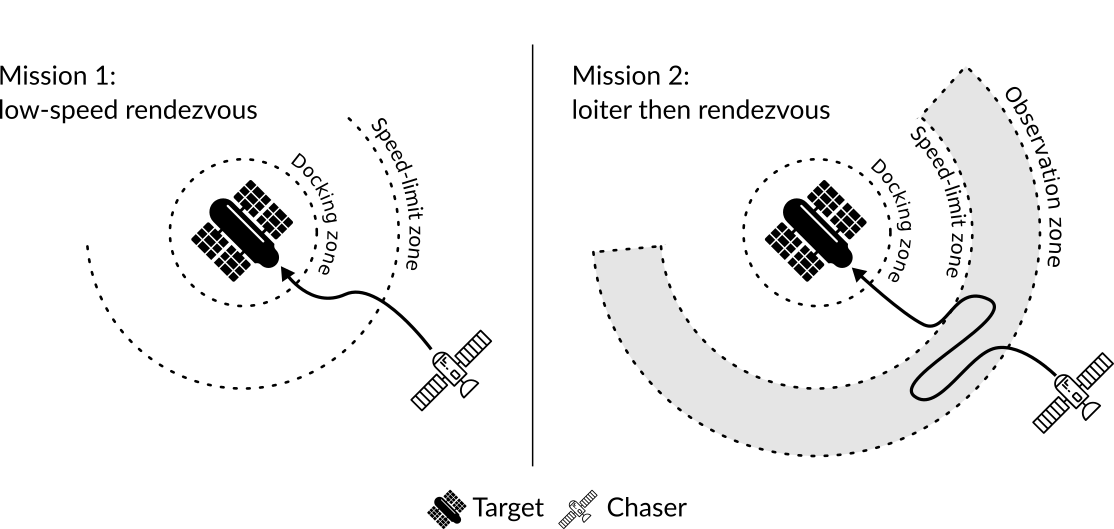
\includegraphics[width=\linewidth]{images/iros/satellite_missions.png}
    \caption{Two satellite rendezvous missions used in our experiments. In the first mission, the chaser satellite must eventually reach the target while respecting a maximum speed constraint in the region immediately around the target. In the second mission, the chaser must still reach the target and obey the speed limit, but it must also loiter in an observation region for some minimum time before approaching. The first mission requires an STL formula with three predicates and three temporal operators, while the second mission requires five predicates and five temporal operators. Figure \textcopyright{} IEEE 2022; used with permission.}
    \label{ch:iros:fig:mission_specs}
\end{figure}

For each mission, the design parameters $\theta$ define the planned trajectory for the chaser (represented as state and input waypoints) as well as the feedback control gains used to track that trajectory, while the exogenous parameters $\phi$ represent bounded uncertainty in the initial state of the chaser ($p_x(0), p_y(0) \in [10, 13]$, $p_z(0) \in [-3, 3]$, $v_x(0), v_y(0), v_z(0) \in [-1, 1]$). We simulate both missions for \SI{200}{s} with a \SI{2}{s} timestep. For each mission, we include a penalty on the total impulse $I$ (in Newton-seconds) required for the maneuver, with $J_\psi = \rho(\psi, S(\theta, \phi), 0) + \lambda I$ and $\lambda = 5\times10^{-5}$.

\subsection{Baselines}

We compare our approach against two baselines: an MIP planner based on that in~\cite{raman15} and~\cite{sadraddiniRobustTemporalLogic2016} and the nonlinear optimization approach from~\cite{pantSmoothOperatorControl2017,pantazidesSatelliteMissionPlanning2022}.

The MIP approach uses a model-predictive control formulation, and~\cite{raman15} proposes to add counterexamples after solving each instance of the problem. Due to the large size of the resulting MIPs (2800-4500 integer variables for these case studies), we could not find an optimal solution for either satellite problem within 1 hour. Because we were not able to solve even a single instance of the MIP planning problem, we were not able to solve it multiple times to generate any MIP-generated counterexamples. For the comparisons below, we take the best feasible solution found after \SI{500}{s} for the first mission and \SI{1000}{s} for the second mission.

We also compare with extensions of the nonlinear optimization method from~\cite{pantSmoothOperatorControl2017,pantazidesSatelliteMissionPlanning2022} that include domain randomization with either 32 or 64 samples of $\phi$. These methods are similar to those proposed in~\cite{leungBackPropagationSignalTemporal2021}, but we re-implement the method to ensure a fair comparison (our implementation uses just-in-time compilation to speed up gradient computation, resulting in a speed increase over the original implementation). We use the same cost function as in our method, with the same penalty on total impulse.

In the following, we denote our method as CG (counterexample-guided), the nonlinear optimization methods as NLopt (with additional notation for the number of domain randomization examples), and the mixed integer programming method as MIP.

\subsection{Results}

Figs.~\ref{ch:iros:fig:mission_1_comparison} and~\ref{ch:iros:fig:mission_2_comparison} show the results of solving the first and second missions, respectively, with each method. In all cases, we compare the results starting the optimization process from 50 random seeds, reporting the time required and the robustness of the optimized plan under an adversarial disturbance computed via local gradient ascent against the optimal solution. Experiments are run on a laptop computer with \SI{8}{GB} of RAM and a \SI{1.8}{GHz} 8-core CPU.

\begin{figure}[tbh]
    \centering
    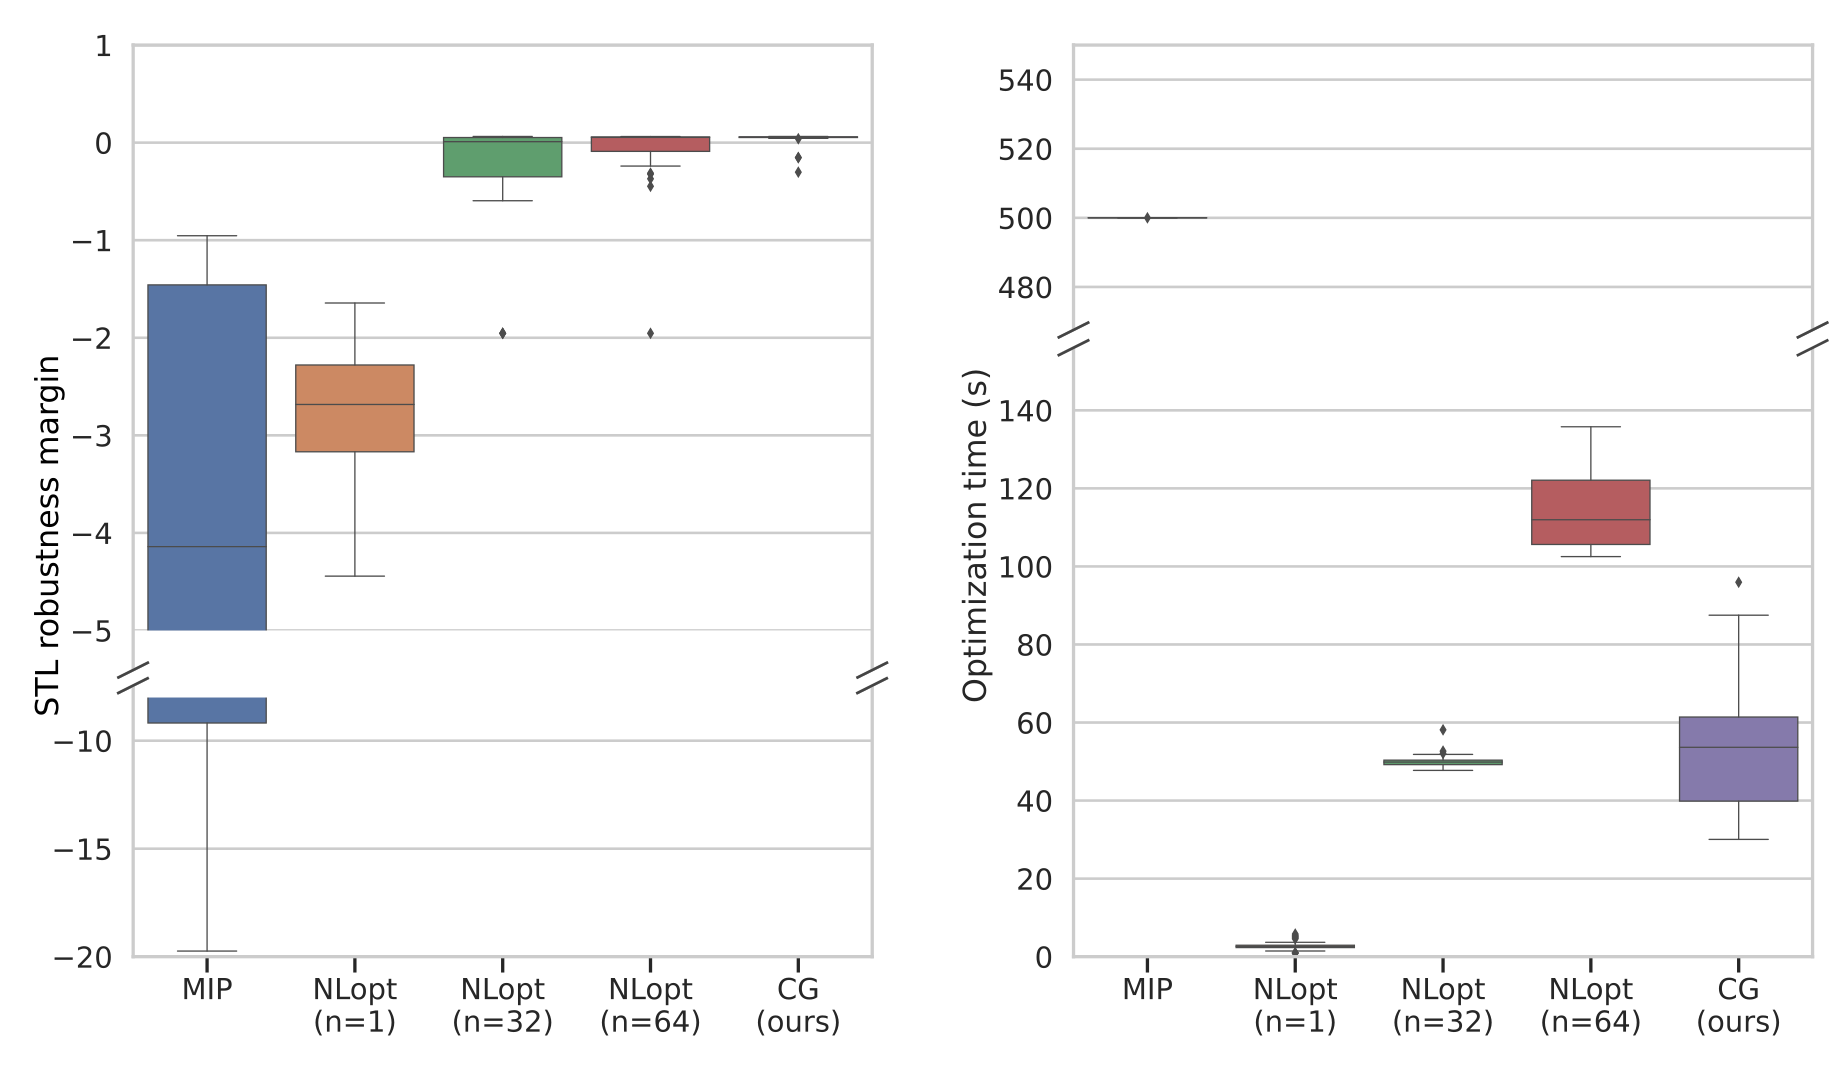
\includegraphics[width=\linewidth]{iros/mission_1_comparison.png}
    \caption{Comparison of different STL planning methods on the first example mission, averaged over 50 random seeds. Left: the robustness margin $\rho(\psi_1)$ computed for the optimized design parameters and worst-case exogenous parameters. Right: the planning time required by each method. Our method (CG) achieves much higher robustness than all other methods (satisfying the STL specification despite adversarial perturbations in all but 3 instances) and runs twice as fast as the next-most-robust method. Figure \textcopyright{} IEEE 2022; used with permission.}
    \label{ch:iros:fig:mission_1_comparison}
\end{figure}

\begin{figure}[tbh]
    \centering
    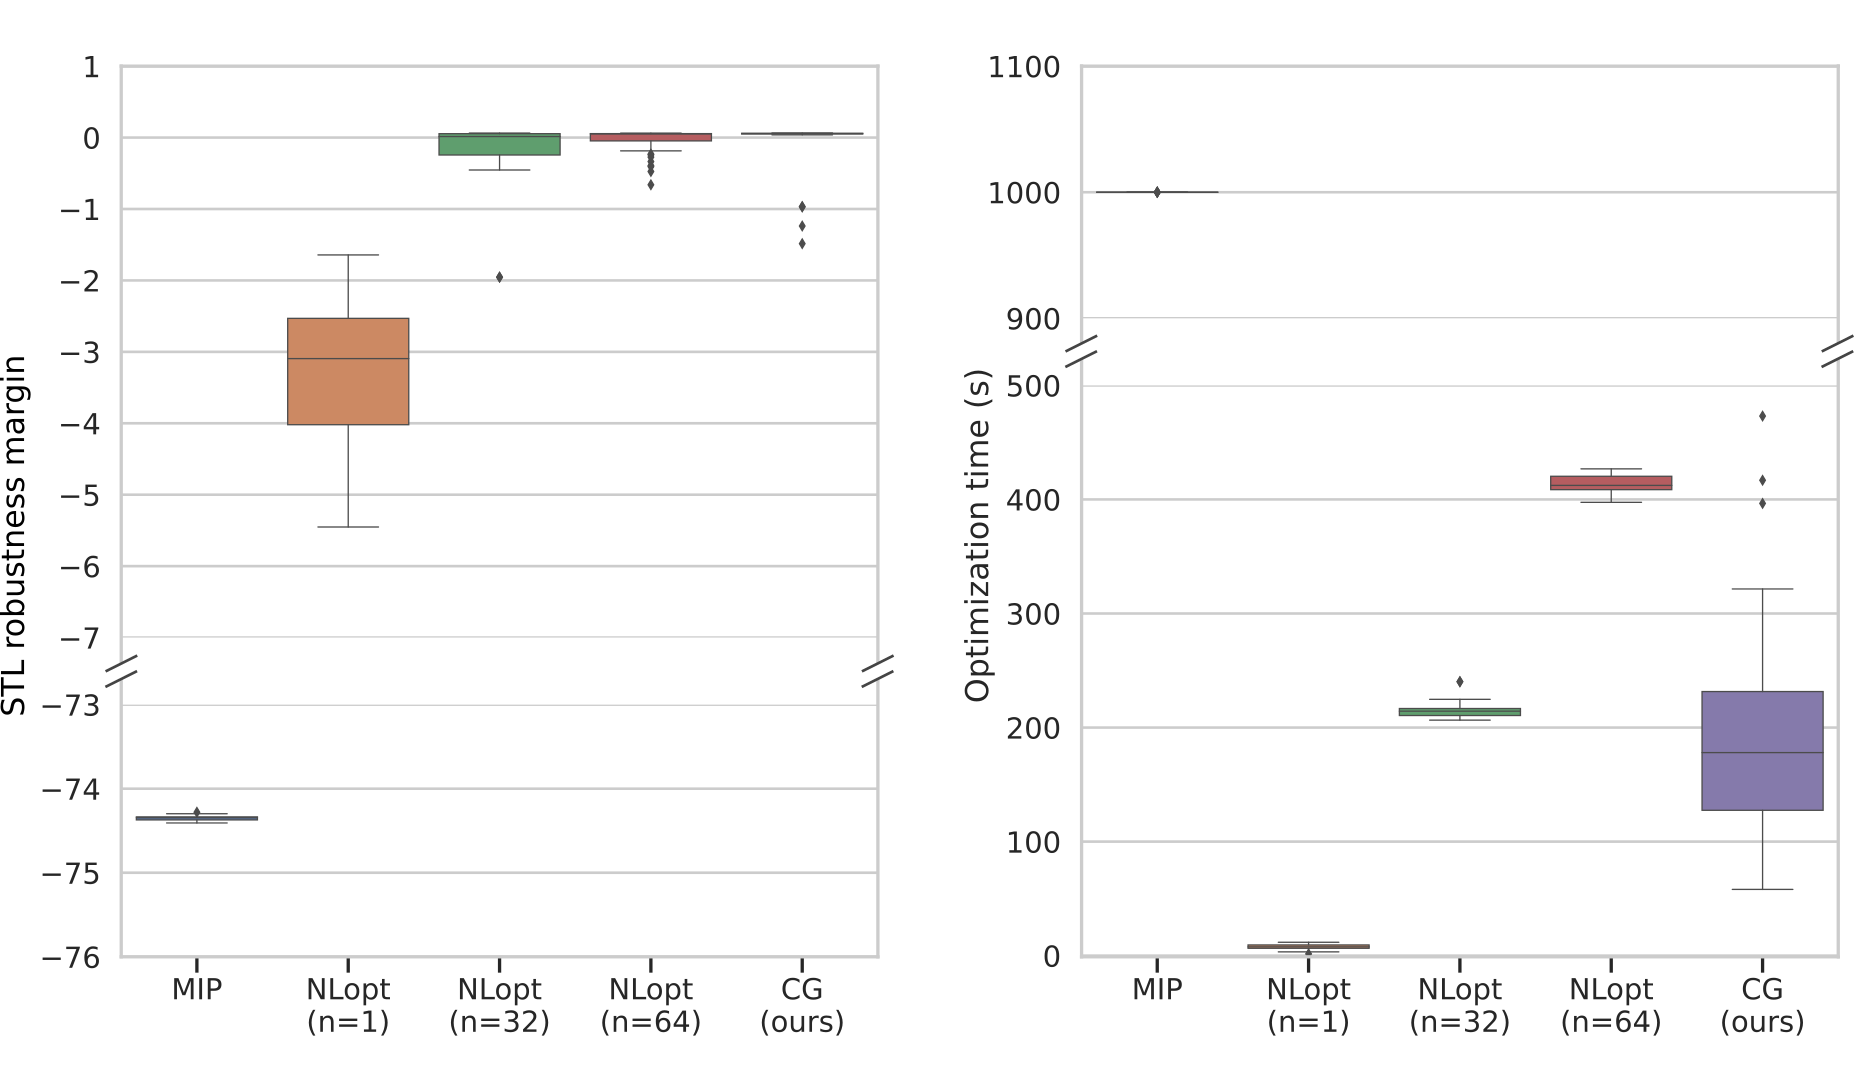
\includegraphics[width=\linewidth]{iros/mission_2_comparison.png}
    \caption{Comparison of different STL planning methods on the second example mission, averaged over 50 random seeds. Left: the robustness margin $\rho(\psi_2)$ computed for the optimized design parameters and worst-case exogenous parameters. Right: time required by each method to find a plan. Our method (CG) finds much more robust plans, satisfying the specification in all but 4 instances compared to 17 failures for the next-best method (NLopt with 64 examples). Our method also runs more than twice as fast as the next-most-robust method. Figure \textcopyright{} IEEE 2022; used with permission.}
    \label{ch:iros:fig:mission_2_comparison}
\end{figure}

Across both missions, we find that our method consistently yields more robust plans than prior methods. In the first mission, our method finds designs that satisfy the STL specifications in all but 3 trials despite the worst-case adversarial disturbance (an example trajectory is shown in Fig.~\ref{ch:iros:fig:mission_1_traj}), while the next-best method (NLopt with 64 domain randomization samples) fails on 14 out of 50 trials and takes more than twice as long to run (\SI{114.3}{s} vs. \SI{53.7}{s} for our method). These results demonstrate the importance of using high-quality counterexamples during optimization: instead of 64 random samples, our method uses 8 initial random samples and 1--4 (median 2) additional counterexamples found using Algorithm~\ref{ch:iros:alg:cg_gs}. Because the MIP cannot practically be solved multiple times to consider variation in $\phi$, the solutions found using the MIP method tend to be less robust; moreover, MIP failed to find a feasible solution for the first mission within \SI{500}{s} in 16 out of 50 trials.

Our method also performs well on the second mission, satisfying the STL requirement on 46 out of 50 random trials; a representative trajectory is shown in Fig.~\ref{ch:iros:fig:mission_2_traj}. Despite an additional \SI{500}{s} of solving time, the MIP method fails to find a feasible solution in $16$ out of 50 trials (the MIP encoding requires 2806 binary variables). The second-most-robust method, after ours, is NLOpt with 64 random examples; this method fails to find a design that satisfies the STL requirement on 17 out of 50 trials despite taking twice as long to run as our method (which required a median of 2 iterations of Algorithm~\ref{ch:iros:alg:cg_gs}).

\begin{figure}[tbh]
    \centering
    \begin{subfigure}[b]{0.45\linewidth}
        \centering
        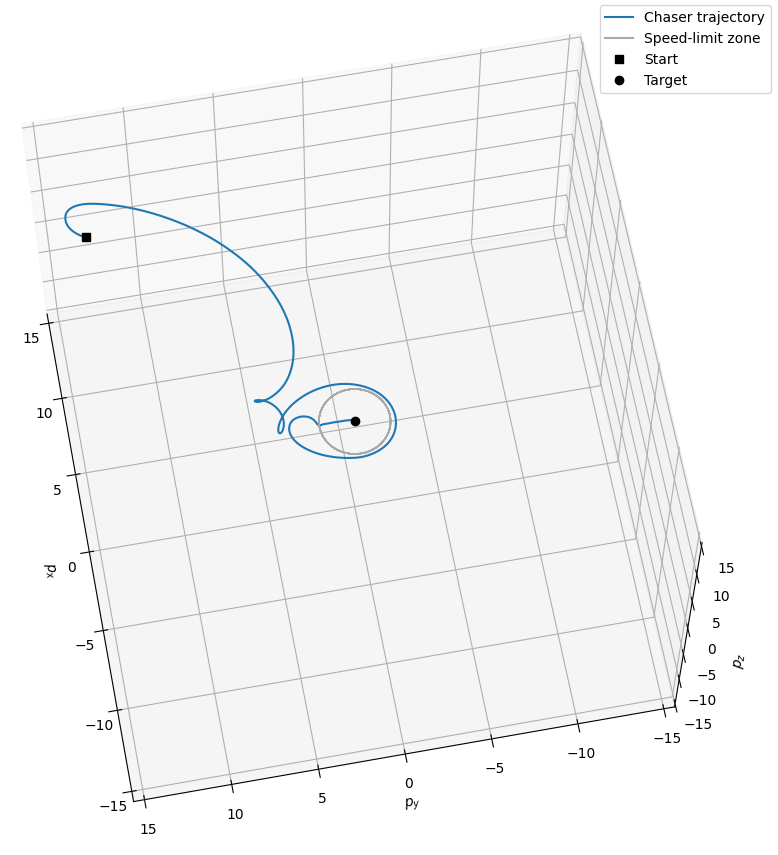
\includegraphics[width=0.9\linewidth]{iros/satellite_mission1_traj.png}
        \caption{Mission 1.}
        \label{ch:iros:fig:mission_1_traj}
    \end{subfigure}
    \quad
    \begin{subfigure}[b]{0.45\linewidth}
        \centering
        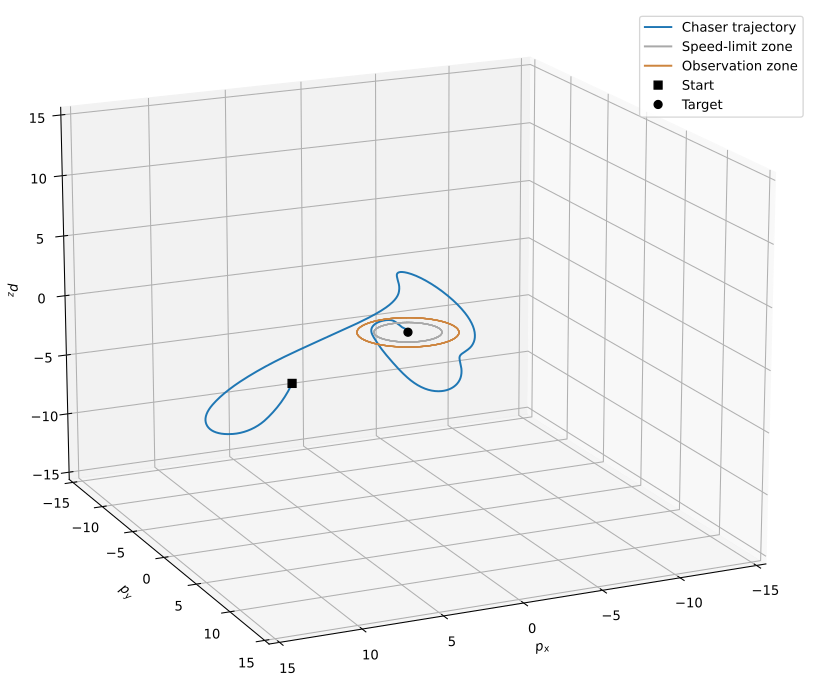
\includegraphics[width=\linewidth]{iros/satellite_mission2_traj.png}
        \caption{Mission 2.}
        \label{ch:iros:fig:mission_2_traj}
    \end{subfigure}
    \caption{Optimized trajectories found using our method for the two satellite rendezvous missions. Figures \textcopyright{} IEEE 2022; used with permission.}
\end{figure}

\section{Summary}

In this chapter, we describe a counterexample-guided approach to end-to-end robot design optimization with formal behavior specifications. This chapter closes two gaps that were left open in Chapter~\ref{ch:rss}. First, by using STL to directly specify the desired behavior, we avoid the need for manual reward design. Second, we consider robustness to worst-case disturbances at design time using counterexample-guided adversarial optimization (rather than the post-hoc statistical method from Chapter~\ref{ch:rss}).

Our empirical results show that our adversarial optimization method yields optimized designs that are more robust than those found by competing methods, despite requiring substantially less computational effort than the next-best method. That said, all methods described in this chapter (aside from intractable MIP-based methods) are inherently local; they rely on local optimization to find both promising designs and adversarial counterexamples. As a result, there is a risk that our method, and any other method that relies on local gradient-based optimization, will get stuck in a local optimum. At first glance, this sub-optimality might not seem like a large issue, since local optimization methods have been successful in many robotics and learning applications~\cite{dawsonCertifiableRobotDesign2022}. Unfortunately, for safety-critical applications, a sub-optimal counterexample is potentially worse than no counterexample at all. This is because a sub-optimal counterexample --- i.e. an artificially easy test case --- can lead to false negatives where we erroneously believe that we have mitigated the worst-case disturbance. We can see this issue manifest in Figs.~\ref{ch:iros:fig:mission_1_comparison} and~\ref{ch:iros:fig:mission_2_comparison} in the few failures that remain even after Algorithm~\ref{ch:iros:alg:cg_gs} converges. In these cases, Algorithm~\ref{ch:iros:alg:cg_gs} has converged to a local Nash equilibrium and has not correctly identified the true worst-case disturbance.

In the next chapter, we will introduce a novel reformulation of the counterexample-guided optimization problem that addresses this issue. By combining (approximately) global probabilistic inference methods with gradients from differentiable simulation, we can find more challenging counterexamples that will lead to correspondingly more robust designs.